%% ------------------------------------------------------------------------- %%
\chapter{Conceitos}
\label{cap:conceitos}


%% ------------------------------------------------------------------------- %%
\section{Perceptrons de Camada Única}\index{área do trabalho!fundamentos}
\label{sec:fundamentos}

  O perceptron é construído em torno de um neurônio não-linear, isto é, o modelo de \textit{MacCulloch-Pitts} de um neurônio. Este modelo de neurônio consite de um combinador linear seguido por um limitador abrupto (realizando a função sinal), como apresentador na Figura \ref{sec:perceptron:model}. O nó aditivo do modelo neuronal caucula uma combinação linear das entradas aplicadas às sua sinapses e também incorpora um bias aplicado externamente. A soma resultante, isto é, o campo local induzido, é aplicado ao limitador abrupto.

\begin{figure}[!htpb] \centering{
  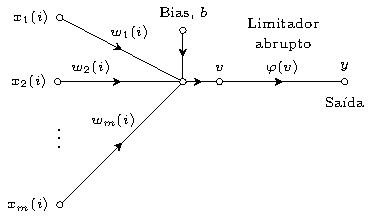
\includegraphics[scale=1]{figuras/perceptron/main.pdf}}
  \caption{Grafo de fluxo do sinal do perceptron}
  \label{sec:perceptron:model}
\end{figure}

\subsection{ Teorema de convergência do perceptron}

Para derivar o algoritmo de aprendizagem por correção de erro para o perceptron, achamos mais conveniente trabalhar com o modelo modificado do grafo de fluxo de sinal da Figura \ref{sec:perceptron:graphmodel}. Neste segundo modelo, que é equivalete àquele da Figura \ref{sec:perceptron:model}, o bias $b(n)$ é tratado como um peso sináptico acionado por uma entrada fixa igual a $+1$. Podemos assim definir o vetor de entrada $(m+1)$-por-$1$
\begin{equation*}
  \textbf{x}(n) = \left[+1,\, x_1(n)\, x_2(n), \cdots,\, x_m(n)\right]^T
\end{equation*}
onde $n$ representa o passo de iteração na aplicação do algoritmo. Correspondentemente, definimos o vetor de pesos $(m+1)$-por-$1$ como
\begin{equation*}
  \textbf{w}(n) = \left[b(n),\, w_1(n)\, w_2(n), \cdots,\, w_m(n)\right]^T
\end{equation*}

Corespondentemente, a saída do combinador linear pode ser escrita na forma compacta
\begin{align}
  \nonumber v(n)&=\sum_{i=0}^{m}w_i(n)x_i(n)\\ 
  &=\textbf{w}^T(n)\textbf{x}(n) \label{sec:perceptron:campolocal}
\end{align}
onde $w_0(n)$ representa o bias $b(n)$. Para $n$ fixo, a equação $\textbf{w}^T\textbf{x}=0$, traçada em um espaço multidimensional (traçada para um bias determinado) com coordenadas $ x_1\, x_2, \cdots,\, x_m$, define um hiperplano como a superfície de decisão entre duas classes diferentes de entradas.

\begin{figure}[!htpb] \centering{
  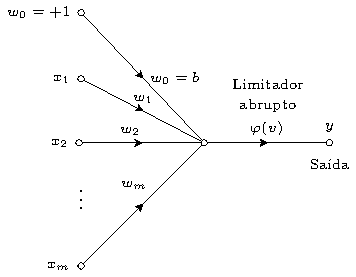
\includegraphics[scale=1]{figuras/perceptronmodel/main.pdf}}
  \caption{Grafo de fluxo do sinal do perceptron}
  \label{sec:perceptron:graphmodel}
\end{figure}

Para o perceptron funcionar corretamente, as duas classes $\mathscr{C}_1$ e $\mathscr{C}_2$ devem ser \textit{linearmente separáveis}. Por sua vez, isto significa que os mpadrões a serem classificados devem estar suficientemente separados entre si para assegurar que a superfície de dicisão consista de um hiperplano.

Suponhamos então que as variáveis de entrada do perceptron se originem de duas classes linearmente separáveis. Seja $\mathscr{X}_1$ o subconjunto de vetores de treinamento $\textbf{x}_1(1),\, \textbf{x}_1(2), \, \cdots $ que pertencem à classe $\mathscr{C}_1$ e seja $\mathscr{X}_2$ o subconjunto de vetores de treinamento $\textbf{x}_2(1),\, \textbf{x}_2(2), \, \cdots $ que pertencem à classe $\mathscr{C}_2$. A união de $\mathscr{X}_1$ e $\mathscr{X}_2$ é o conjunto de treinamento completo $\mathscr{X}$. Dados os conjuntos de vetores $\mathscr{X}_1$ e $\mathscr{X}_2$ para treinar o classificador, o processo de treinamento envolve o ajuste de peso $\textbf{w}$ de tal forma que as duas classes $\mathscr{C}_1$ e $\mathscr{C}_2$ sejam linearmente separáveis. Isto é, existe um vetor de peso $\textbf{w}$ para o qual podemos afirmar

\begin{equation}
  \begin{aligned} \label{sec:perceptron:classes}
    \textbf{w}^T\textbf{x} &> 0 \text{ para todo vetor de entrada $\textbf{x}$ pertencente à classe  $\mathscr{C}_1$} \\       
    \textbf{w}^T\textbf{x} &\leq 0 \text{ para todo vetor de entrada $\textbf{x}$ pertencente à classe  $\mathscr{C}_2$}
  \end{aligned}
\end{equation}
Na segunda linha da Equação \ref{sec:perceptron:classes}, escolhemos arbitrariamente que o vetor de entrada $\textbf{x}$ pertence à classe $\mathscr{C}_2$ se $\textbf{w}^T\textbf{x}=0$. Dados os sobconjuntos de vetores de treinamento $\mathscr{X}_1$ e $\mathscr{X}_2$, o problema de treinamento para o perceptron elementar é, então, encontrar um vetor de peso $\textbf{w}$ tal que as duas desigualdades da Equação \ref{sec:perceptron:classes} sejam satisfeitas.

O algoritmo para adaptar o vetor de peso do perceptron elementar pode ser formulado como segue:

\begin{enumerate}
  \item Se o $n$-ésimo membro do conjunto de treinamento, $\textbf{x}(n)$, é corretamente classificado pelo vetor de peso $\textbf{w}(n)$ calculado na $n$-ésima iteração do algoritmo, então o vetor de peso do perceptron não é corrigido de acordo com a regra:
  \begin{equation}
    \begin{aligned} \label{sec:perceptron:alg1}
      \textbf{w}(n+1) &= \textbf{w}(n)\quad \text{ se $\textbf{w}^T(n)\textbf{x}(n) > 0 $ e $\textbf{x}(n)$ pertencente à classe  $\mathscr{C}_1$} \\
      \textbf{w}(n+1) &= \textbf{w}(n)\quad \text{ se $\textbf{w}^T(n)\textbf{x}(n) \leq 0 $ e $\textbf{x}(n)$ pertencente à classe  $\mathscr{C}_2$} 
    \end{aligned}
  \end{equation}
  \item Caso contrário, o vetor de peso do percptron é atualizado de acordo com a regra
    \begin{equation}
      \begin{aligned} \label{sec:perceptron:alg2}
        \textbf{w}(n+1) &= \textbf{w}(n) - \eta (n)\textbf{x}(n)\quad \text{ se $\textbf{w}^T(n)\textbf{x}(n) > 0 $ e $\textbf{x}(n)$ pertencente à classe  $\mathscr{C}_2$} \\
        \textbf{w}(n+1) &= \textbf{w}(n) + \eta (n)\textbf{x}(n)\quad \text{ se $\textbf{w}^T(n)\textbf{x}(n) \leq 0 $ e $\textbf{x}(n)$ pertencente à classe  $\mathscr{C}_1$} 
      \end{aligned}
    \end{equation}
\end{enumerate}
onde o \textit{parâmetro da taxa de aprendizagem} $\eta (n)$ controla o ajuste aplicado ao vetor de peso na iteração $n$.

\noindent
Se $\eta(n)=\eta>0$, onde $\eta$ é uma constante independente do número da iteração $n$, temos uma \textit{regra de adaptação com incremento fixo} para o perceptron.

No que segue, primeiro provamos a convergência de uma regra de adaptação com incremento fixo para a qual $\eta=1$. Claramente, o valor de $\eta$ não é importante, desde que seja positivo. Um valor de $\eta \neq 1$ meramente escala os vetores de padrões sem afetar a sua separabilidade.

A prova é apresentada para a condição inicial $\textbf{w}(0)=\textbf{0}$. Suponhamos que $\textbf{w}^T(n)\textbf{x}(n) < 0 $ para $n=1,\, 2,\,\cdots$, e que o vetor de entrada $\textbf{x}(n)$ pertença ao sbconjunto $\mathscr{X}_1$. Isto é, o perceptron classifica incorretamente os vetores $\textbf{x}(1),\,\textbf{x}(2),\,\cdots$, já que a segunda condição da Equação \ref{sec:perceptron:classes} é violada. Então, com a constante $\eta(n)=1$, podemos a segunda linha da Equação \ref{sec:perceptron:alg2} para escrever
\begin{equation}\label{sec:perceptron:weightplus}
  \textbf{w}(n+1)=\textbf{w}(n)+\textbf{x}(n)\quad \text{para $\textbf{x}(n)$ pertencente à classe $\mathscr{C}_1$.}
\end{equation}
Dada a condição inicial $\textbf{w}(0)=\textbf{0}$, podemos resolver iterativamente esta equação para $\textbf{w}(n+1)$ obtendo o resultado
\begin{equation}\label{sec:perceptron:weightplusint}
  \textbf{w}(n+1)=\textbf{x}(1)+\textbf{x}(2)+\cdots+\textbf{x}(n)
\end{equation}
Como as classes $\mathscr{C}_1$ e $\mathscr{C}_2$ são assumidas como sendo linearmnete separáveis, existe uma solução $\textbf{w}_0$ para a qual $\textbf{w}^T(n)\textbf{x}(n)>0$ para os vetores $\textbf{x}(1),\,\cdots,\,\textbf{x}(n)$ pertencentes ao subconjunto $\mathscr{X}_1$. Para uma solução fixa $\textbf{w}_0$, podemos então definir um número positivo $\alpha$ como
\begin{equation}\label{sec:perceptro:alphamin}
  \alpha = \min_{\textbf{x}(n)\in \mathscr{X}_1}\textbf{w}_0^T\textbf{x}(n)
\end{equation}
Assim, multiplicando ambos os lados da Equação \ref{sec:perceptron:weightplusint} pelo vetor linha $\textbf{w}_0^T$, obtemos
\begin{equation*}
  \textbf{w}_0^T\textbf{w}(n+1)=\textbf{w}_0^T\textbf{x}(1)+\textbf{w}_0^T\textbf{x}(2)+\cdots+\textbf{w}_0^T\textbf{x}(n)
\end{equation*}
Consequentemente, com base na definição dada na Equação \ref{sec:perceptro:alphamin}, temos
\begin{equation*}
  \textbf{w}_0^T\textbf{w}(n+1) \geq n\alpha
\end{equation*}
Da \textit{desigualdade de Cauchy-Schwarz} segue que
\begin{equation*}
  \Vert \textbf{w}_0\Vert^2\Vert \textbf{w}(n+1) \Vert^2\geq n^2\alpha^2
\end{equation*}
ou de forma equivalente,
\begin{equation}\label{sec:perceptron:firsteq}
  \Vert \textbf{w}(n+1) \Vert^2\geq \frac{n^2\alpha^2}{\Vert \textbf{w}_0\Vert^2}
\end{equation}
A seguir, seguimos com um outro caminho de desenvolvimento. Em particular, reescrevemos a Equação \ref{sec:perceptron:weightplus} na forma
\begin{equation}\label{sec:perceptron:weightplusmodified}
  \textbf{w}(k+1)=\textbf{w}(k)+\textbf{x}(k)\quad \text{para $k=1,\,\cdots,\,n$ e $\textbf{x}(k)\in \mathscr{X}_1$}
\end{equation}
Calculando a morma euclidiana quadrática de ambos os lados da Equação \ref{sec:perceptron:weightplusmodified}, obtemos
\begin{equation}\label{sec:perceptron:weightplusnormed}
  \Vert \textbf{w}(k+1) \Vert^2= \Vert \textbf{w}(k) \Vert^2+\Vert \textbf{x}(k) \Vert^2+2\textbf{w}^T(k)\textbf{x}(k)
\end{equation}
Mas, sob a suposição que o perceptron classifica incorretamente um vetor de entrada $\textbf{x}(k)$ pertencente ao subconjunto $\mathscr{X}_1$, temos $\textbf{w}^T(k)\textbf{x}(k)<0$. Consequentemente, deduzimos da Equação \ref{sec:perceptron:weightplusnormed} que
\begin{equation*}\label{sec:perceptron:weightplusnormeddiff}
  \Vert \textbf{w}(k+1) \Vert^2- \Vert \textbf{w}(k) \Vert^2\leq  \Vert \textbf{x}(k) \Vert^2, \quad k=1,\,\cdots,\, n
\end{equation*}
Somando estas desigualdades para $k=1,\cdots,\, n$ e invocando a condição inicial assumida $\textbf{w}(0)=\textbf{0}$, obtemos a desigualdade:
\begin{equation}
  \begin{aligned} \label{sec:perceptron:weightplussecond}
    \Vert \textbf{w}(k+1) \Vert^2 &\leq \sum_{k=1}^n \Vert \textbf{x}(k) \Vert^2\\
    &\leq n\beta
  \end{aligned}
\end{equation}
onde $\beta$ é um número positivo definido por
\begin{equation}\label{sec:perceptron:beta}
  \beta=\max_{\textbf{x}(k)\in\mathscr{X}_1}\Vert\textbf{x}(k)\Vert^2
\end{equation}
A Equação \ref{sec:perceptron:weightplussecond} afirma que a norma euclidana quadrática do vetor de peso $\textbf{w}(n+1)$ cresce no máximo linearmente como o número de iterações $n$.
  O segundo resultado da Equação \ref{sec:perceptron:weightplussecond} está claramente em conflito com o resultado anterior da Equação \ref{sec:perceptron:firsteq} para valores suficientemente grandes de $n$. De fato, podemos afirmar que $n$ não pode ser maior que um valor $n_{\rm max}$ para o qual as Equações \ref{sec:perceptron:firsteq} \ref{sec:perceptron:weightplussecond} são ambas satisfeitas com um sinal de igualdade. Isto é, dada uma solução $\textbf{w}_0$ temos
  \begin{equation}\label{sec:perceptron:nmax}
    n_{\rm max}=\frac{\beta\Vert\textbf{w}_0\Vert^2}{\alpha^2}
  \end{equation}
  Provamos assim que para $\eta(n)=1$ para todo $n$, e $\textbf{w}(0)=\textbf{0}$, e desde que exista um vetor solução $\textbf{w}_0$, a regra para adaptar os pesos sinápticos do perceptron deve terminar após no máximo $n_{\rm max}$ iterações. Note também que das Equações \ref{sec:perceptro:alphamin}, \ref{sec:perceptron:beta} e \ref{sec:perceptron:nmax} que não existe uma solução única para $\textbf{w}_0$ ou $n_{\rm max}$.



  \begin{figure}[!htpb] \centering{
    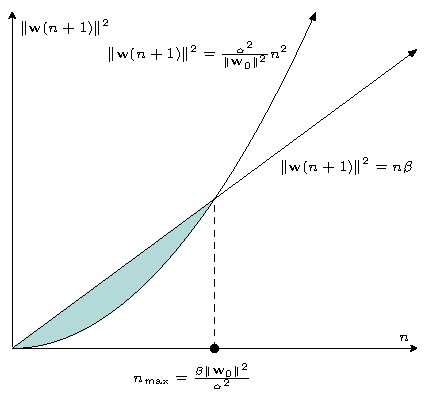
\includegraphics[scale=1]{figuras/perceptrondemo/main.pdf}}
    \caption{Número máximo de iterações}
    \label{sec:perceptron:demo}
  \end{figure}

  \floatname{algorithm}{Procedure}
  \renewcommand{\algorithmicrequire}{\textbf{Input:}}
  \renewcommand{\algorithmicensure}{\textbf{Output:}}

  \begin{algorithm}
    \caption{Algoritmo de convergência do perceptron} 
    \begin{algorithmic}[1]
      \State $\textbf{X}_1\leftarrow$ Entradas pertencentes à classe $\mathscr{X}_1$
      \State $\textbf{X}_2\leftarrow$ Entradas pertencentes à classe $\mathscr{X}_2$
      \State Inicialize $\textbf{w}$ com zeros
      \While {$!convergence$}
      \State Escolha aleatoriamente $\textbf{x}\in\textbf{X}_1\cup \textbf{X}_2$ 

      \If {$\textbf{x}\in\textbf{X}_1$ e $\textbf{w}\cdot\textbf{x}<0$}
      \State $\textbf{w} = \textbf{w} + \textbf{x}$
      \EndIf

      \If {$\textbf{x}\in\textbf{X}_2$ e $\textbf{w}\cdot\textbf{x}\geq 0$}
      \State $\textbf{w} = \textbf{w} -  \textbf{x}$
      \EndIf

      \EndWhile
      % \For {$iteration=1,2,\ldots$}
      %   \For {$actor=1,2,\ldots,N$}
      %     \State Run policy $\pi_{\theta_{old}}$ in environment for $T$ time steps
      %     \State Compute advantage estimates $\hat{A}_{1},\ldots,\hat{A}_{T}$
      %   \EndFor
      %   \State Optimize surrogate $L$ wrt. $\theta$, with $K$ epochs and minibatch size $M\leq NT$
      %   \State $\theta_{old}\leftarrow\theta$
      % \EndFor
    \end{algorithmic} 
  \end{algorithm}

  \section{Perceptrons de Múltiplas Camadas}



